\documentclass[UTF8]{ctexart}

%固定图片位置
\usepackage{float}

%插入超链接
\usepackage{url}

\usepackage{tikz,mathpazo}
\usetikzlibrary{shapes.geometric, arrows}
\usetikzlibrary{calc}


\usepackage{listings}
%插入代码的配置
\definecolor{CPPLight}  {HTML} {686868}
\definecolor{CPPSteel}  {HTML} {888888}
\definecolor{CPPDark}   {HTML} {262626}
\definecolor{CPPBlue}   {HTML} {4172A3}
\definecolor{CPPGreen}  {HTML} {487818}
\definecolor{CPPBrown}  {HTML} {A07040}
\definecolor{CPPRed}    {HTML} {AD4D3A}
\definecolor{CPPViolet} {HTML} {7040A0}
\definecolor{CPPGray}  {HTML} {B8B8B8}
\lstset{
	language=Python,                                     % 设置语言
    columns=fixed,    
    breaklines = true,   
    basicstyle=\small ,
    numbers=left,                                        % 在左侧显示行号
    %frame=none,                                          % 不显示背景边框
    backgroundcolor=\color[RGB]{245,245,244},            % 设定背景颜色
    keywordstyle=\color[RGB]{40,40,255},                 % 设定关键字颜色
    numberstyle=\tiny\color{darkgray},           % 设定行号格式
    %commentstyle=\it\color[RGB]{0,96,96},                % 设置代码注释的格式
    stringstyle=\rmfamily\slshape\color[RGB]{128,0,0},   % 设置字符串格式
    showstringspaces=false,                              % 不显示字符串中的空格                           
    %morekeywords={True,alignas,continute,friend,register,true,alignof,decltype,goto,
    %reinterpret_cast,try,asm,defult,if,return,typedef,auto,delete,inline,short,
    %typeid,bool,do,int,signed,typename,break,double,long,sizeof,union,case,
    %dynamic_cast,mutable,static,unsigned,catch,else,namespace,static_assert,using,
    %char,enum,new,static_cast,virtual,char16_t,char32_t,explict,noexcept,struct,
    %void,export,nullptr,switch,volatile,class,extern,operator,template,wchar_t,
    %const,false,private,this,while,constexpr,float,protected,thread_local,
    %const_cast,for,public,throw,std,rand},
    emph={access,and,break,class,continue,def,del,elif ,else,%
	except,exec,finally,for,from,global,if,import,in,i s,%
	lambda,not,or,pass,print,raise,return,try,while},
    emphstyle=\color{CPPViolet}, 
    emph={[2]True, False, None, self},
	emphstyle=[2]\color{green},
	emph={[3]from, import, as},
	emphstyle=[3]\color{blue},
	upquote=true,
	morecomment=[s]{"""}{"""},
	commentstyle=\color{orange}\slshape,
	emph={[4]1, 2, 3, 4, 5, 6, 7, 8, 9, 0},
	emphstyle=[4]\color{red},
	emph={[5]numpy, np, plt},
	emphstyle=[5]\color{red},
	literate=*{:}{{\textcolor{blue}:}}{1}%
	{=}{{\textcolor{blue}=}}{1}%
	{-}{{\textcolor{blue}-}}{1}%
	{+}{{\textcolor{blue}+}}{1}%
	{*}{{\textcolor{blue}*}}{1}%
	{!}{{\textcolor{blue}!}}{1}%
	{(}{{\textcolor{blue}(}}{1}%
	{)}{{\textcolor{blue})}}{1}%
	{[}{{\textcolor{blue}[}}{1}%
	{]}{{\textcolor{blue}]}}{1}%
	{<}{{\textcolor{blue}<}}{1}%
	{>}{{\textcolor{blue}>}}{1},%
	framexleftmargin=0.1mm, framextopmargin=0.1mm, frame=shadowbox, rulesepcolor=\color{black},
}



\usepackage{geometry}
\geometry{left=2cm, right=2cm, top=1.2cm, bottom=1.2cm}

%得到引用的标题内容
\usepackage{nameref} 

%添加首行缩进,两个字符
\usepackage{indentfirst}
\setlength{\parindent}{2em}

%多行公式一个编号
\usepackage{amsmath}

%文献引用,标准类型为plain
%\usepackage[hyperref=true,backend=biber,sorting=none,backref=true]{biblatex}
%\addbibresource{ref.bib}
\bibliographystyle{plain}
\usepackage{cite}

\pagestyle{plain}

%跨页表格
\usepackage{multirow}
\usepackage{longtable,booktabs}
\usepackage{supertabular}
\usepackage{makecell}

%调整itemize等的间距
\usepackage{enumitem}


\usepackage{graphicx}

%超链接
\usepackage[linkcolor=yellow,citecolor=red,backref=page,hyperfootnotes=true]{hyperref}
\hypersetup{
bookmarks=true,
colorlinks=true,
linkcolor=black
}
\usepackage{tabularx} %This package must be placed after package {hyperref}, otherwise footnote marks are NOT treated as hyperlinks.


%引入了一些改进的数学环境,如align
\usepackage{amsmath}

\title{数据结构:list ADT}
\author{姓名:鲁国锐 \protect\newline
\and 学号:17020021031 \\
\and 专业:电子信息科学与技术}


\begin{document}
	\maketitle
	\renewcommand{\contentsname}{Contents}
	\tableofcontents
	\newpage
	
	\hypersetup{
	bookmarks=true,
	colorlinks=true,
	linkcolor=red,
	urlcolor=blue
	}
	\section{问题分析}
	\subsection{题目描述}
	\indent 自己编写$list$ $ADT$,调试并完成下面内容。注:本次作业不允许使用$c++$标准模版库。
	\begin{itemize}[leftmargin=60pt]
	
	\item 任务一:
	\begin{itemize}
		\item[$\circ$] 实现$PrintLots(L,P)$,并分析运行时间。
		\item[$\circ$] 有两个链表$L$和$P$, 他们包含以升序排列的整数。操作$PrintLots(L,P)$将打印$L$中那些由$P$所指定位置上的元素。如:$P={1,3,4,6}$, 则,$L$中第$1$,第$3$,第$4$,第$6$个元素被打印出来。
	\end{itemize}
		

	\item 任务二:懒惰删除
	\begin{itemize}
		\item[$\circ$] 列出懒惰删除的优点和缺点
		\item[$\circ$] 编写实现
		
		不同于我们已经给出的删除方法,另一种是使用懒惰删除($lazy\ deletion$)。为了删除一个元素,我们只标记上该元素被删除。表中被删除和非被删除元素的个数作为数据结构的一部分被保留。如果被删除元素和非被删除元素一样多,我们遍历整个表,对所有被标记的节点执行标准的删除算法。
	\end{itemize}			
	\end{itemize}
	

	\subsection{问题分析}
	\indent 根据题目,我们需要解决的问题有:
	\begin{enumerate}[leftmargin=50pt]

	\item 编写$Node$和$List$类,包括实现$List$中一系列必须的成员函数,如:构造函数、析构函数、$insert$函数、$remove$函数等(见\ref{desigh_class}节);
	\item 设计输入输出流程(见\ref{design_input_and_output}节);
	\item 实现$PrintLots$函数(见\ref{PrintLots}节)和$lazy\ deletion$函数(见\ref{lazy_del}节)及其相关的部分函数;
	\item 分析$PrintLots$的时间复杂度(见\ref{time_of_PrintLots}节);
	\item 分析懒惰删除的有点和缺点(见\ref{adv_and_disadv_of_lazy_deletion}节)。
	\end{enumerate}
	

	
	\section{解决方案}
		\subsection{编写$Node$类和$List$类}\label{desigh_class}
			\indent 我们首先要写$Node$类,它的属性包括值$val$、指向前驱的指针$pred$、指向后继的指针$succ$以及在本题中需额外设置的一个属性$deleted$,用以表示该节点是否被标记为删除。其构造函数相对简单,在此不做赘述。
			
			\indent 接下来是$List$类,它的属性包括头指针$header$、尾指针$trailer$、长度$\_size$(不包括头指针和尾指针)和被标记为删除的元素个数$\_delNum$。至于其成员函数(参考教材\cite{data_structure}),由于数量较多,我们只用一表格列出,并做简要说明。
			\begin{center}
			\begin{longtable}[H]{|c|c|c|c|}
            \caption{$List$成员函数}
            \label{functions}
			\\
			\hline
			\textbf{函数名}&\textbf{输入}&\textbf{输出}&\textbf{说明} \\
			\hline
			\endfirsthead
			
			\hline
			\textbf{函数名}&\textbf{输入}&\textbf{输出}&\textbf{说明} \\
			\hline
			\endhead
			
			\hline
			\multicolumn{4}{|c|}{\textsl{下页继续}} \\
			\hline
			\endfoot
			
			\hline
			\endlastfoot
			
			\hline
			构造函数&无&无&初始化整个链表,建立头结点和尾节点 \\			
				
			\hline
			析构函数&无&无&删除链表,释放内存 \\			
			
			\hline
			$insert$&指针$r$,值$e$&该节点的指针&在$r$所指向的节点之前插入一个节点 \\
			
			\hline
			$push\_back$&值$e$&无&在尾节点之前插入一个结点 \\
			\hline
			
			$remove$&指针$r$&被删除节点下一个节点的指针&\makecell{删除$r$指向的节点} \\
			\hline
			
			$clear$&无&被删除元素的个数&清空链表(不包括头结点和尾节点)\\
			\hline
			
			$clear\_mark$&无&无&\makecell{调用$remove$函数清除所有被标记为\\已删除的节点} \\
			\hline
			
			$lazeDel$&指针$r$&被删除元素的值&\makecell{用懒惰删除的方式删除$r$指向的节点} \\
			\hline
			
			$getP$&序号(从$1$开始计数)&指向序号所对应的节点的指针&将输入的序号转换为指针,方便后续的操作 \\
			\hline 
			
			$print$&无&无&\makecell{输出链表中所有节点的值\\(不包括头结点和尾节点)} \\
			\hline
			
			$getHeader$&无&头指针&返回头指针 \\
			\hline
			
			$getTrailer$&无&尾指针&返回尾指针 \\
			\hline 
			
			$size$&无&\makecell{链表长度\\(不包括头结点和尾节点)}&返回链表长度(不包括头结点和尾节点) \\
			\hline

			\end{longtable}			
			\end{center}
		
		
		\subsection{设计输入输出流程}\label{design_input_and_output}
		\indent 我们首先输入链表$L$各节点的值,这些值以空格分隔,以回车结束。然后通过三条指令来控制这个程序的流程:
			\begin{itemize}[leftmargin=50pt]
			\item $delete$:执行懒惰删除操作,后跟一数字表示要删除节点的序号;
			\item $PrintLots$:调用$PrintLots$函数,后跟一组以空格分隔的数字,表示链表$P$中各节点的元素;
			\item $end$:结束整个程序。
			\end{itemize}
			
		\indent 每次执行完$delete$或$PrintsLots$后,把$L$中各节点的值输出一遍。其中在执行$PrintLots$时还会把$P$以及$L$中对应于$P$所表示的序号的节点值输出一遍,分别以“$P:$”和“$L:$”开头。
		
		\subsection{实现$PrintLots$函数}\label{PrintLots}
		\indent 有了表\ref{functions}中的各个函数,我们实现$PrintLots$就会轻松不少。
		
		\indent 首先我们要检查$L$是否为空,若为空则直接结束函数的调用。若不为空,我们开始执行输出操作。这里定义了两个指针$pl$和$pp$,分别初始化为指向$L$的头节点和$P$的第一个节点。同时为了避免在得到$P$中节点的值后要从头开始遍历$L$,我们还需定义两个整型变量$pre$和$offset$。其中$pre$中记录的是$P$中前一个节点的值,而$offset$中记录的则是$pl$需要向后移动的位数。每次我们令$pp$向后移动一位,然后用$pp$指向的节点中的值减去$pre$,所得结果赋给$offset$,然后令$pl$向后移$offset$位,输出其对应节点中的值。
		
		\indent 另外在执行输出操作时我们还要不断检查$pl$是否越界。如果发现$pl$指向了尾节点,立马抛出异常并结束整个函数。
		\subsection{实现$lazy\ deletion$函数}\label{lazy_del}
		\indent 这个函数实现起来相对简单。我们只需要把传入指针对应的节点中$deleted$属性置为$true$即可。同时还要将链表中的$\_delNum$加一。然后判断$\frac{\_size}{2} \leq \_delNum$是否成立。若成立,则执行$clear_mark$函数,将链表中所有$deleted$为$true$的节点删除,并把$\_delNum$值$0$。
	\section{算法设计}
	见图\ref{to RPN}、图\ref{main}。


\begin{figure}[H]
	\centering 
	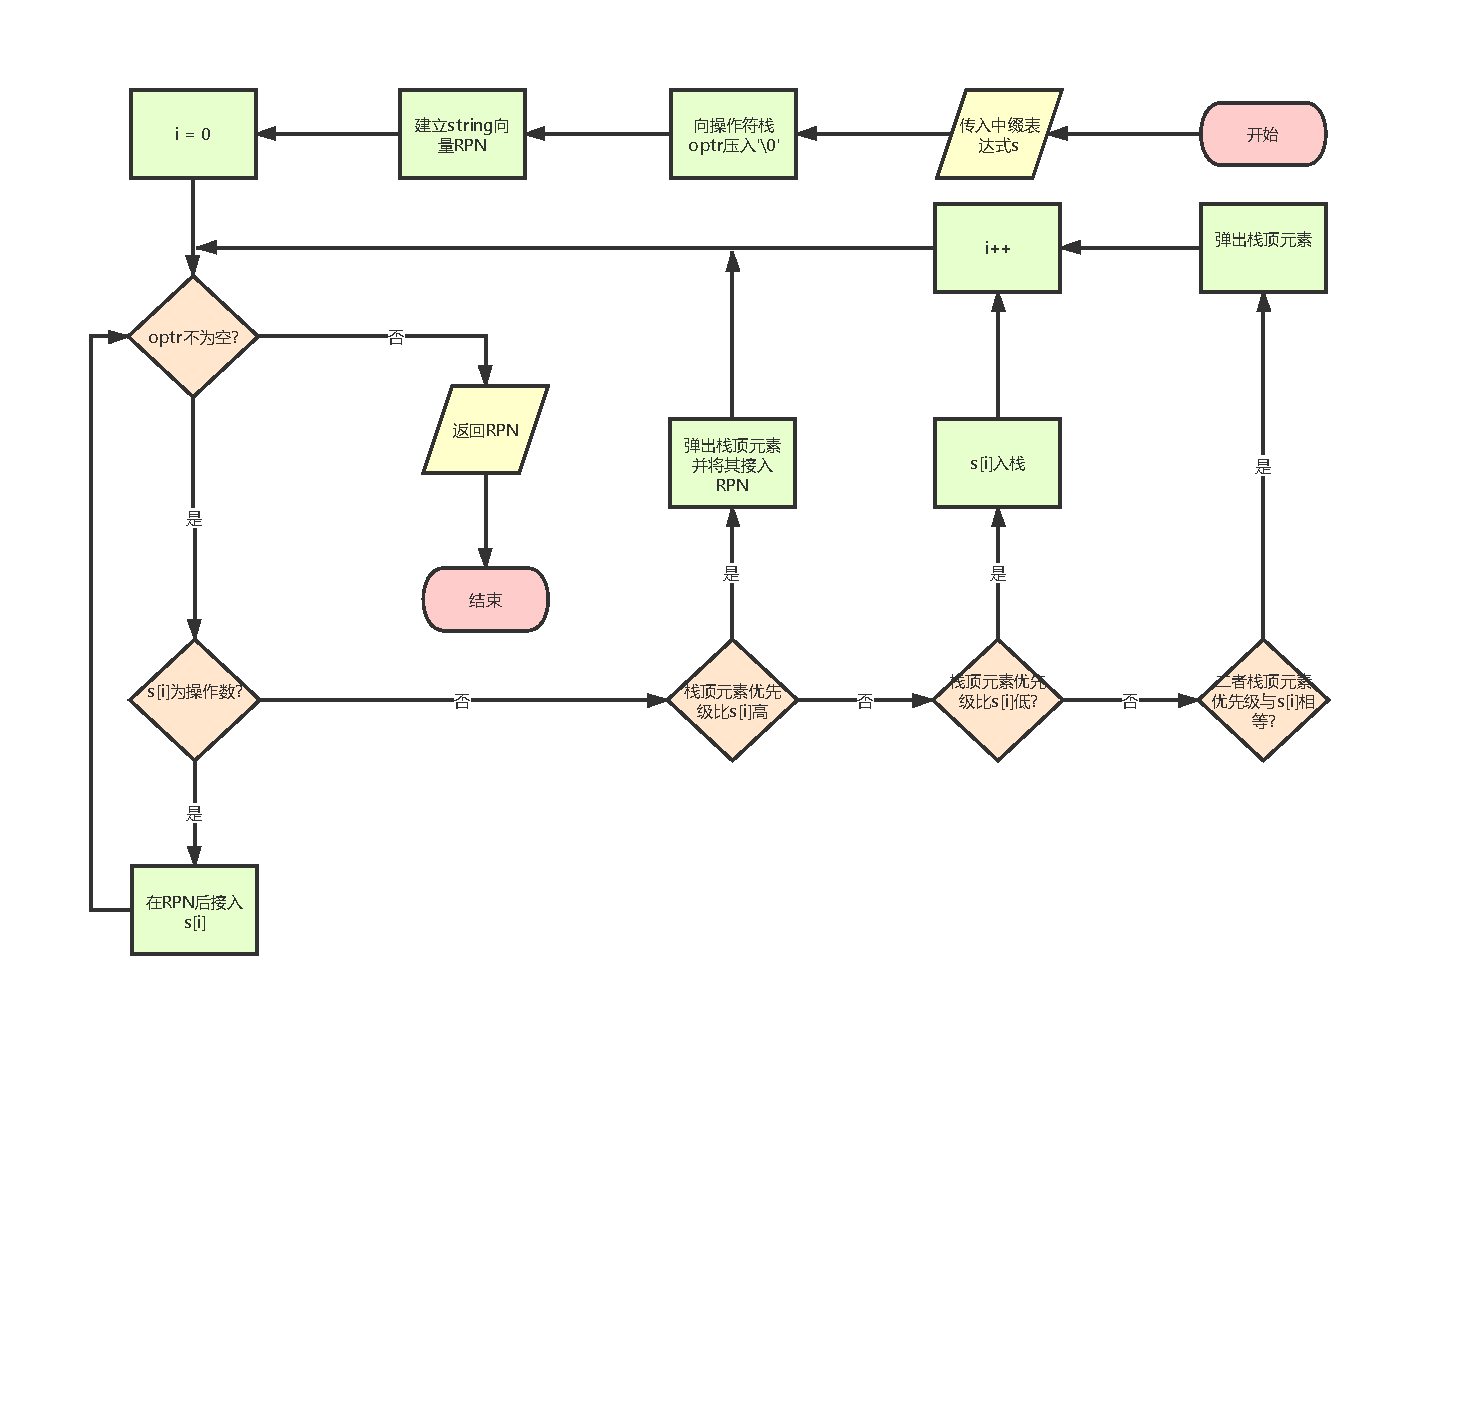
\includegraphics[width=20cm, height=19cm]{to_RPN.pdf} 
	\caption{$to_RPN$函数流程图} 
	\label{to RPN}
\end{figure}



\begin{figure}[H]
	\centering 
	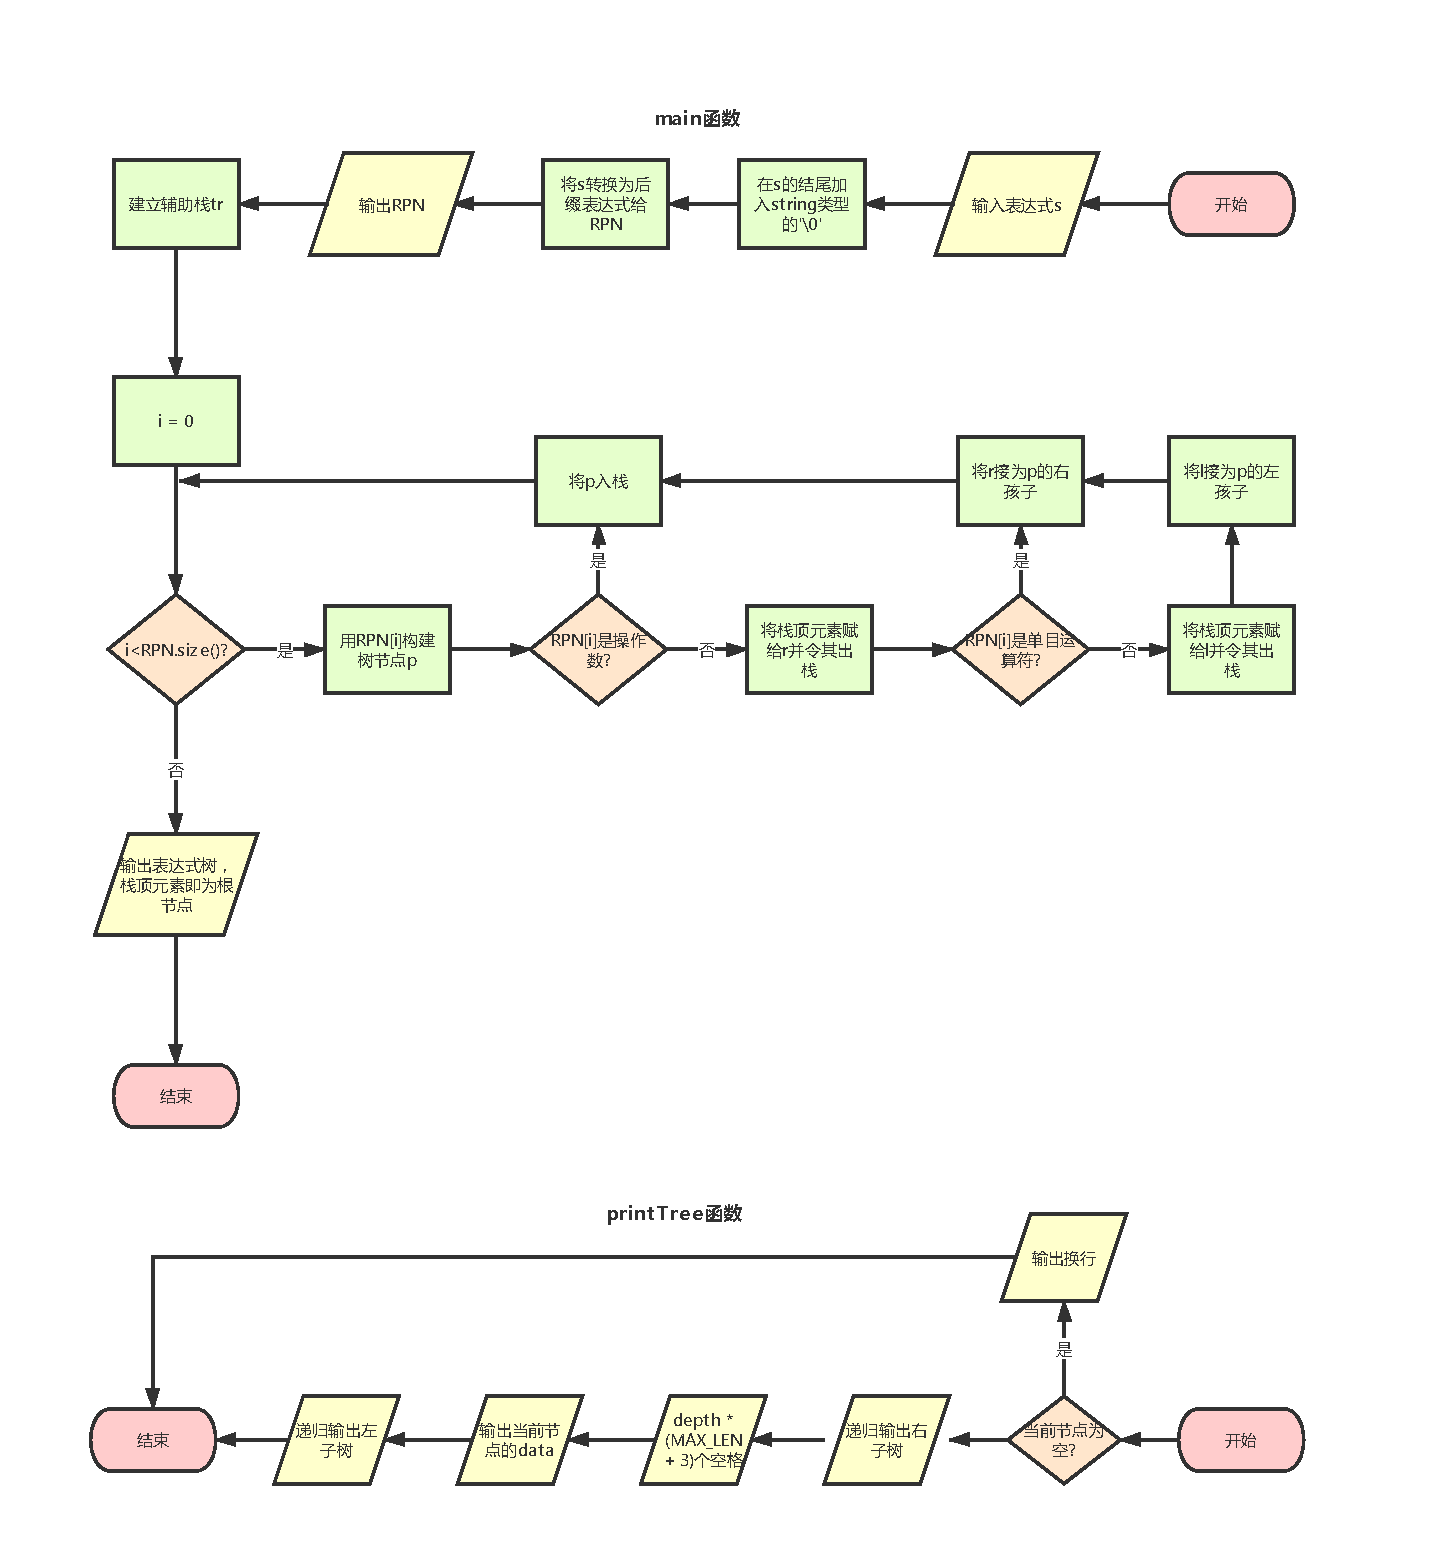
\includegraphics[width=20cm, height=23cm]{expression_tree_main.pdf} 
	\caption{$main$函数流程图} 
	\label{main}
\end{figure}
\newpage



	\section{编程实现\protect \footnotemark[1]}
	\footnotetext[1]{代码也可从该网址得到:\url{https://github.com/chenfeng123456/CourseInOUC/blob/master/algorithm/expression_tree/expression_tree.cpp}}

	\begin{lstlisting}[language=C++,caption={expression\_tree代码},label={expression_tree_code}]
#include <iostream>
#include <string>
#include <stack>
#include <vector>
#include <typeinfo>
#include <map>


using namespace std;
#define N_OPTR 9
typedef enum { ADD, SUB, MUL, DIV, POW, FAC, L_P, R_P, EOE } Operator;
//             +    -    *    /    ^    !    (    )    \0

const char pri[N_OPTR][N_OPTR] =
{
'>',   '>',   '<',   '<',   '<',   '<',   '<',   '>',   '>',
'>',   '>',   '<',   '<',   '<',   '<',   '<',   '>',   '>',
'>',   '>',   '>',   '>',   '<',   '<',   '<',   '>',   '>',
'>',   '>',   '>',   '>',   '<',   '<',   '<',   '>',   '>',
'>',   '>',   '>',   '>',   '>',   '<',   '<',   '>',   '>',
'>',   '>',   '>',   '>',   '>',   '>',   ' ',   '>',   '>',
'<',   '<',   '<',   '<',   '<',   '<',   '<',   '=',   ' ',
' ',   ' ',   ' ',   ' ',   ' ',   ' ',   ' ',   ' ',   ' ',
'<',   '<',   '<',   '<',   '<',   '<',   '<',   ' ',   '='
};


#define IsRoot ( !((x).parent))
#define IsLc(x) ( ! IsRoot(x) && ( &(x) == (x).parent->lc))
#define IsRc(x) ( ! IsRoot(x) && ( &(x) == (x).parent->rc))
//#define FromParentTo(x) (IsRoot(x)

char order(string a, string b)
{
static map<string, int> symbols;
symbols["+"] = ADD;
symbols["-"] = SUB;
symbols["*"] = MUL;
symbols["/"] = DIV;
symbols["^"] = POW;
symbols["!"] = FAC;
symbols["("] = L_P;
symbols[")"] = R_P;
symbols["\0"] = EOE;

return pri[symbols[a]][symbols[b]];
}

template <typename T>
class Node
{
public:
T data;
Node<T> *parent;
Node<T> *lc;
Node<T> *rc;
int height;

Node() : parent(NULL), lc(NULL), rc(NULL), height(0) {}
Node(T e, Node<T> *p=NULL, Node<T> *l=NULL, Node<T> *r=NULL, int h=0) :
data(e), parent(p), lc(l), rc(r), height(h) {}
Node<T> *insertAsLc(Node<T> *e);
Node<T> *insertAsRc(Node<T> *e);
};
template <typename T>
Node<T>* Node<T>::insertAsLc(Node<T> *e)
{
lc = e;
e->parent = this;
return e;
}
template <typename T>
Node<T>* Node<T>::insertAsRc(Node<T> *e)
{
rc = e;
e->parent = this;
return e;
}



template <typename T>
void travPost(Node<T> *x)
{
if (!x) return;
travPost(x->lc);
travPost(x->rc);
cout << x->data << " ";
}

bool isdigit(string s)
{
if ((s[0] >= '0' && s[0] <= '9') || (s[0] >= 'a' && s[0] <= 'z'))
return true;
return false;
}

vector<string>& toRPN(vector<string> s)
{
static vector<string> RPN;
//stack<string> opnd;
stack<string> optr;
optr.push("\0");
int i = 0;
while (!optr.empty())
{
//cout << endl;
//cout << "i = " << i << endl;
//cout << "RPN = " << RPN << endl;
//cout << "optr.size() = " << optr.size() << endl;
if (i >= s.size())
break;
if (isdigit(s[i]))
{
RPN.push_back(s[i]);
i++;
}
else
{
switch (order(optr.top(), s[i]))
{
case '<':
{
//cout << '<' << endl;
optr.push(s[i]);
i++;
break;
}
case '=':
{
//cout << '=' << endl;
optr.pop();
i++;
break;
}
case '>':
{
//cout << '>' << endl;
string op = optr.top();
optr.pop();
RPN.push_back(op);
//i++;
break;
}
}
}
}

return RPN;
}


template <typename T>
void rm(Node<T> *x)
{
if (!x) return;
rm(x->lc);
rm(x->rc);
delete x;
}

template <typename T>
void remove(Node<T> *x)
{
if (x->parent)
{
if (x == x->parent->lc)
x->parent->lc = NULL;
if (x == x->parent->rc)
x->parent->rc = NULL;
}
rm(x);
}


int main()
{

vector<string> s;

string c;
while(cin >> c)
{
s.push_back(c);
}
s.push_back("\0");
vector<string> RPN = toRPN(s);

for (int i=0; i < RPN.size(); i++)
cout << RPN[i] << " ";
cout << endl;

stack<Node<string>*> tr;
for (int i=0; i < RPN.size(); i++)
{
string temp_op = RPN[i];
Node<string> *p = new Node<string>(temp_op);
if (isdigit(temp_op))
tr.push(p);
else
{
//cout << RPN[i] << "   " << tr.size() << endl;
Node<string> *r = tr.top();
tr.pop();
// For unary operator such as "!".
// If they are placed at the second place
// then we shouldn't perform the operation
// of top() or pop() on the tr. Otherwise,
// it will be runtime error.
Node<string> *l;
if (!tr.empty())
l = tr.top();
if (temp_op != "!")
{
tr.pop();
}
p->insertAsRc(r);
if (temp_op != "!") p->insertAsLc(l);
tr.push(p);
}
}

//cout << "tr.size() = " << tr.size() << endl;
travPost(tr.top());
cout << endl;
return 0;
}

	\end{lstlisting}
	
	\section{结果分析}
	\subsection{结果展示}
	\newpage
\begin{figure}[H]
	\centering 
	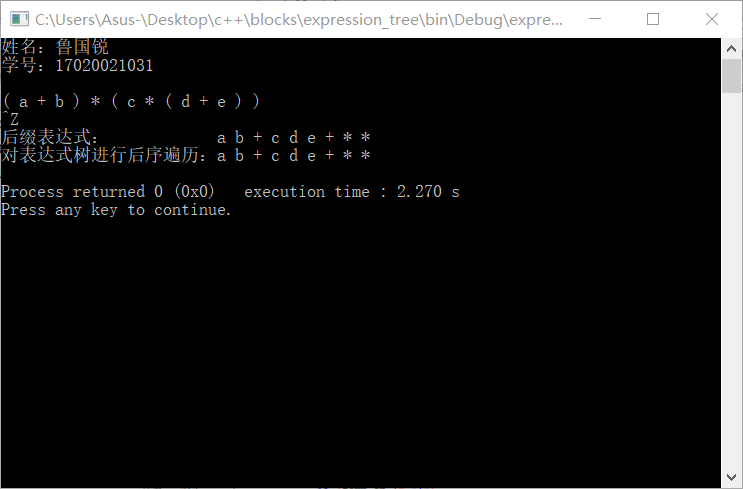
\includegraphics[scale=0.85]{res1.png} 
	\caption{结果1} 
	\label{res1}
\end{figure}

\begin{figure}[H]
	\centering 
	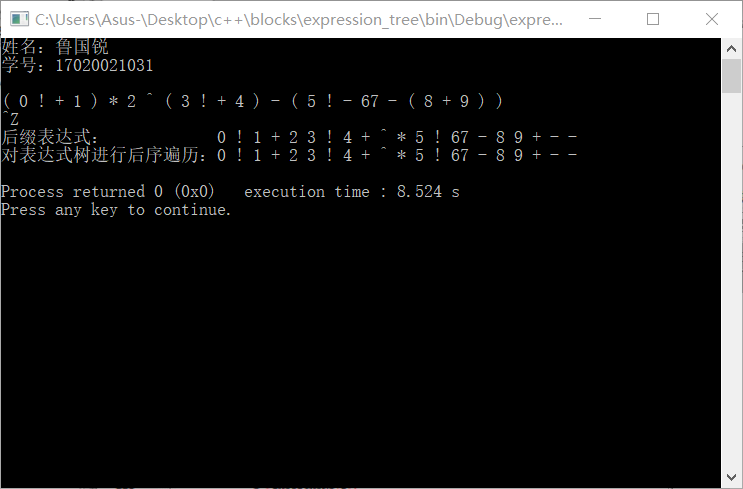
\includegraphics[scale=0.85]{res2.png} 
	\caption{结果2} 
	\label{res2}
\end{figure}

\begin{figure}[H]
	\centering 
	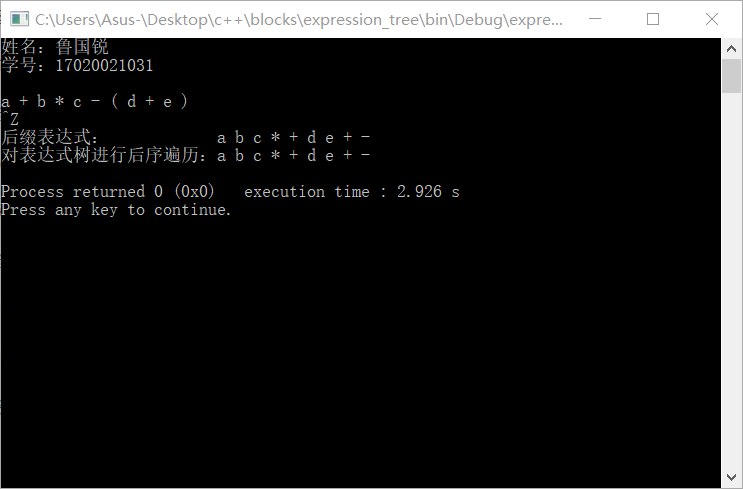
\includegraphics[scale=0.85]{res3.png} 
	\caption{结果3} 
	\label{res3}
\end{figure}

\begin{figure}[H]
	\centering 
	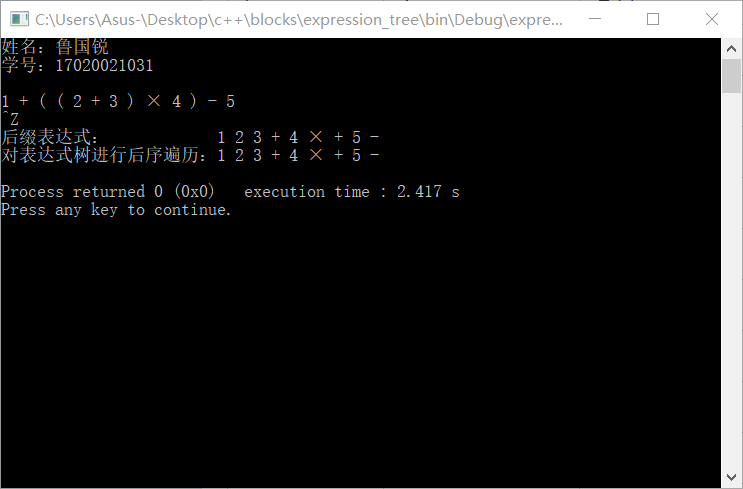
\includegraphics[scale=0.85]{res4.png} 
	\caption{结果4} 
	\label{res4}
\end{figure}

	\subsection{$PrintLots$运行时间}\label{time_of_PrintLots}
	\indent 由于我们在执行输出操作时引入$pre$和$offset$两个变量从而避免了对$L$的重复遍历。因此,即使在最坏情况下,即需要输出$L$中的最后一个元素时,我们也只需令$pl$向后移动$L.\_size$次,所需时间与$L$的长度成正比。故其时间复杂度为$O(N)$。
	
	\subsection{懒惰删除的优点和缺点}\label{adv_and_disadv_of_lazy_deletion}
	\indent 懒惰删除的优点:
	\begin{itemize}[leftmargin=50pt]
	\item 减少删除节点时所需的时间;
	\item 避免频繁地对内存进行操作;
	\item 简化代码复杂程度;
	\item 在对被删除位置进行插入时\textbf{可能}会减少时间。
	\end{itemize}
	
	\indent 懒惰删除的缺点:
	\begin{itemize}[leftmargin=50pt]
	\item 会占用更多的空间;
	\item 由于在链表中由于并没有真正删除节点,所以会增减遍历链表所需的时间;
	\end{itemize}
	\section{总结体会}
	\indent 在完成这次作业的过程中,由于一开始没有加入检查指针是否越界的代码,导致在调试过程中因指针越界使得电脑死机了,从而不得不强制关机重启。这次的教训让我更深刻地明白了检查指针越界的重要性,同时还促使我去学习了如何在$C++$中捕获异常并输出错误信息。
	\indent 另外还没有完全解决的一点是,因为我不想在输入链表的值之前还要输入长度,所以采取的做法是当检测到输入数字后跟的是回车时就跳出循环。但如果在输入回车之前不小心多输入了空格,
并在输入回车后输入命令,也会使电脑几乎陷入死机状态。我暂时还没想出是什么原因导致的,也没有很好的解决方法。

\bibliography{ref.bib}
\end{document}